\hypertarget{interfaceDataFactory}{
\section{Data\-Factory  Interface Reference}
\label{interfaceDataFactory}\index{DataFactory@{Data\-Factory}}
}
Inheritance diagram for Data\-Factory:\begin{figure}[H]
\begin{center}
\leavevmode
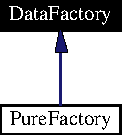
\includegraphics[width=47pt]{interfaceDataFactory__inherit__graph}
\end{center}
\end{figure}
\subsection*{Public Methods}
\begin{CompactItemize}
\item 
\hyperlink{interfaceEmpty}{Empty} \hyperlink{interfaceDataFactory_a0}{make\-Empty} ()
\item 
\hyperlink{interfaceData}{Data} \hyperlink{interfaceDataFactory_a1}{make\-Tuple} (\hyperlink{interfaceDataValue}{Data\-Value} data\-Value, \hyperlink{interfaceData}{Data} data)
\item 
\hyperlink{interfaceInt}{Int} \hyperlink{interfaceDataFactory_a2}{make\-Int} (long n)
\item 
\hyperlink{interfaceToken}{Token} \hyperlink{interfaceDataFactory_a3}{make\-Token} (String s)
\item 
\hyperlink{interfaceBool}{Bool} \hyperlink{interfaceDataFactory_a4}{make\-Bool} (boolean b)
\item 
\hyperlink{interfaceMessageTag}{Message\-Tag} \hyperlink{interfaceDataFactory_a5}{make\-Message\-Tag} (String s)
\item 
\hyperlink{interfaceList}{List} \hyperlink{interfaceDataFactory_a6}{make\-List1} (\hyperlink{interfaceDataValue}{Data\-Value} data\-Value)
\item 
\hyperlink{interfaceList}{List} \hyperlink{interfaceDataFactory_a7}{make\-List0} ()
\item 
\hyperlink{interfaceAction}{Action} \hyperlink{interfaceDataFactory_a8}{make\-Action} (\hyperlink{interfaceEnactable}{Enactable} enactable)
\item 
\hyperlink{interfaceBindings}{Bindings} \hyperlink{interfaceDataFactory_a9}{make\-No\-Bindings} ()
\item 
\hyperlink{interfaceAgent}{Agent} \hyperlink{interfaceDataFactory_a10}{make\-Agent} ()
\item 
\hyperlink{interfaceCell}{Cell} \hyperlink{interfaceDataFactory_a11}{make\-Cell} ()
\end{CompactItemize}


\subsection{Member Function Documentation}
\hypertarget{interfaceDataFactory_a8}{
\index{DataFactory@{Data\-Factory}!makeAction@{makeAction}}
\index{makeAction@{makeAction}!DataFactory@{Data\-Factory}}
\subsubsection[makeAction]{\setlength{\rightskip}{0pt plus 5cm}\hyperlink{interfaceAction}{Action} Data\-Factory::make\-Action (\hyperlink{interfaceEnactable}{Enactable} {\em enactable})}}
\label{interfaceDataFactory_a8}




Reimplemented in \hyperlink{classPureFactory_a12}{Pure\-Factory}.\hypertarget{interfaceDataFactory_a10}{
\index{DataFactory@{Data\-Factory}!makeAgent@{makeAgent}}
\index{makeAgent@{makeAgent}!DataFactory@{Data\-Factory}}
\subsubsection[makeAgent]{\setlength{\rightskip}{0pt plus 5cm}\hyperlink{interfaceAgent}{Agent} Data\-Factory::make\-Agent ()}}
\label{interfaceDataFactory_a10}




Reimplemented in \hyperlink{classPureFactory_a8}{Pure\-Factory}.

Referenced by Schedule::Schedule(), and Schedule::activate().

\hypertarget{interfaceDataFactory_a4}{
\index{DataFactory@{Data\-Factory}!makeBool@{makeBool}}
\index{makeBool@{makeBool}!DataFactory@{Data\-Factory}}
\subsubsection[makeBool]{\setlength{\rightskip}{0pt plus 5cm}\hyperlink{interfaceBool}{Bool} Data\-Factory::make\-Bool (boolean {\em b})}}
\label{interfaceDataFactory_a4}




Reimplemented in \hyperlink{classPureFactory_a3}{Pure\-Factory}.\hypertarget{interfaceDataFactory_a11}{
\index{DataFactory@{Data\-Factory}!makeCell@{makeCell}}
\index{makeCell@{makeCell}!DataFactory@{Data\-Factory}}
\subsubsection[makeCell]{\setlength{\rightskip}{0pt plus 5cm}\hyperlink{interfaceCell}{Cell} Data\-Factory::make\-Cell ()}}
\label{interfaceDataFactory_a11}




Reimplemented in \hyperlink{classPureFactory_a9}{Pure\-Factory}.

Referenced by Store::create().

\hypertarget{interfaceDataFactory_a0}{
\index{DataFactory@{Data\-Factory}!makeEmpty@{makeEmpty}}
\index{makeEmpty@{makeEmpty}!DataFactory@{Data\-Factory}}
\subsubsection[makeEmpty]{\setlength{\rightskip}{0pt plus 5cm}\hyperlink{interfaceEmpty}{Empty} Data\-Factory::make\-Empty ()}}
\label{interfaceDataFactory_a0}




Reimplemented in \hyperlink{classPureFactory_a10}{Pure\-Factory}.

Referenced by Schedule::deactivate(), Tagged\-Buffers::dequeue(), Store::destroy(), Store::inspect(), Schedule::receive(), Schedule::send(), and Store::update().

\hypertarget{interfaceDataFactory_a2}{
\index{DataFactory@{Data\-Factory}!makeInt@{makeInt}}
\index{makeInt@{makeInt}!DataFactory@{Data\-Factory}}
\subsubsection[makeInt]{\setlength{\rightskip}{0pt plus 5cm}\hyperlink{interfaceInt}{Int} Data\-Factory::make\-Int (long {\em n})}}
\label{interfaceDataFactory_a2}




Reimplemented in \hyperlink{classPureFactory_a1}{Pure\-Factory}.

Referenced by Schedule::choose\-Natural(), and Schedule::give\-Current\-Time().

\hypertarget{interfaceDataFactory_a7}{
\index{DataFactory@{Data\-Factory}!makeList0@{makeList0}}
\index{makeList0@{makeList0}!DataFactory@{Data\-Factory}}
\subsubsection[makeList0]{\setlength{\rightskip}{0pt plus 5cm}\hyperlink{interfaceList}{List} Data\-Factory::make\-List0 ()}}
\label{interfaceDataFactory_a7}




Reimplemented in \hyperlink{classPureFactory_a5}{Pure\-Factory}.\hypertarget{interfaceDataFactory_a6}{
\index{DataFactory@{Data\-Factory}!makeList1@{makeList1}}
\index{makeList1@{makeList1}!DataFactory@{Data\-Factory}}
\subsubsection[makeList1]{\setlength{\rightskip}{0pt plus 5cm}\hyperlink{interfaceList}{List} Data\-Factory::make\-List1 (\hyperlink{interfaceDataValue}{Data\-Value} {\em data\-Value})}}
\label{interfaceDataFactory_a6}




Reimplemented in \hyperlink{classPureFactory_a6}{Pure\-Factory}.\hypertarget{interfaceDataFactory_a5}{
\index{DataFactory@{Data\-Factory}!makeMessageTag@{makeMessageTag}}
\index{makeMessageTag@{makeMessageTag}!DataFactory@{Data\-Factory}}
\subsubsection[makeMessageTag]{\setlength{\rightskip}{0pt plus 5cm}\hyperlink{interfaceMessageTag}{Message\-Tag} Data\-Factory::make\-Message\-Tag (String {\em s})}}
\label{interfaceDataFactory_a5}




Reimplemented in \hyperlink{classPureFactory_a4}{Pure\-Factory}.\hypertarget{interfaceDataFactory_a9}{
\index{DataFactory@{Data\-Factory}!makeNoBindings@{makeNoBindings}}
\index{makeNoBindings@{makeNoBindings}!DataFactory@{Data\-Factory}}
\subsubsection[makeNoBindings]{\setlength{\rightskip}{0pt plus 5cm}\hyperlink{interfaceBindings}{Bindings} Data\-Factory::make\-No\-Bindings ()}}
\label{interfaceDataFactory_a9}




Reimplemented in \hyperlink{classPureFactory_a7}{Pure\-Factory}.\hypertarget{interfaceDataFactory_a3}{
\index{DataFactory@{Data\-Factory}!makeToken@{makeToken}}
\index{makeToken@{makeToken}!DataFactory@{Data\-Factory}}
\subsubsection[makeToken]{\setlength{\rightskip}{0pt plus 5cm}\hyperlink{interfaceToken}{Token} Data\-Factory::make\-Token (String {\em s})}}
\label{interfaceDataFactory_a3}




Reimplemented in \hyperlink{classPureFactory_a2}{Pure\-Factory}.\hypertarget{interfaceDataFactory_a1}{
\index{DataFactory@{Data\-Factory}!makeTuple@{makeTuple}}
\index{makeTuple@{makeTuple}!DataFactory@{Data\-Factory}}
\subsubsection[makeTuple]{\setlength{\rightskip}{0pt plus 5cm}\hyperlink{interfaceData}{Data} Data\-Factory::make\-Tuple (\hyperlink{interfaceDataValue}{Data\-Value} {\em data\-Value}, \hyperlink{interfaceData}{Data} {\em data})}}
\label{interfaceDataFactory_a1}




Reimplemented in \hyperlink{classPureFactory_a11}{Pure\-Factory}.

The documentation for this interface was generated from the following file:\begin{CompactItemize}
\item 
\hyperlink{DataFactory_8java-source}{Data\-Factory.java}\end{CompactItemize}
